
%(BEGIN_QUESTION)
% Copyright 2015, Tony R. Kuphaldt, released under the Creative Commons Attribution License (v 1.0)
% This means you may do almost anything with this work of mine, so long as you give me proper credit

Electrical {\it transformers} are extensively used in AC power grid systems, the point being to transmit electrical power over long distances at high voltage levels and low current levels so as to limit the size of the metal conductor wires (i.e. cheaper and lighter wiring) and then step voltage down to safer levels (while boosting current) at the points of use.  Transformers installed at large electrical generating stations (``power plants'') step up voltage from the generator level (tens of kilovolts) to the transmission level (hundreds of kilovolts).  Substation transformers step the voltage back down to the tens-of-kilovolts level for distribution through neighborhoods, and finally distribution transformers step the voltage down once more to household and business levels (120, 240, and/or 480 volts).

\vskip 10pt

Determine the following about this power distribution transformer, such as the kind seen on power poles near homes and businesses in the United States:

$$\includegraphics[width=15.5cm]{i04754x01.eps}$$

\begin{itemize}
\item{} How can we tell from the schematic diagram that this transformer is a voltage {\it step-down} unit?
\vskip 10pt 
\item{} The meaning of the ``240/120'' designation.
\vskip 10pt 
\item{} The amount of current through the fuse at a customer load of 11 kW.
\end{itemize}



\vskip 20pt \vbox{\hrule \hbox{\strut \vrule{} {\bf Suggestions for Socratic discussion} \vrule} \hrule}

\begin{itemize}
\item{} Why do you suppose the secondary winding of this power transformer is center-tapped?
\item{} What purpose does it serve to build AC power distribution systems with transformers in them to step voltages up and down at different locations?  Why not just build a power system with a consistent voltage level everywhere?
\item{} Only one fuse is shown on the high-voltage side of this transformer circuit.  What does the lack of a second fuse tell us about the two high-voltage powerline conductors?
\end{itemize}

\underbar{file i04754}
%(END_QUESTION)





%(BEGIN_ANSWER)

\noindent
{\bf Partial answer:}

\begin{itemize}
\item{} The fact that this is a {\bf step-down} transformer, is clearly evident from its primary/secondary turns ratio: the winding having more turns will exhibit greater voltage (and less current) than the winding having fewer turns
\vskip 10pt 
\item{} Fuse current = 1.528 amps
\end{itemize}

%(END_ANSWER)





%(BEGIN_NOTES)

This is a {\bf step-down} transformer, because the primary winding has more turns than the secondary.

\vskip 10pt

The ``240/120'' designation refers to the center-tapped secondary winding, and how it provides both 120 VAC and 240 VAC to the customer.  The middle terminal is customarily grounded to earth and called the {\it neutral} conductor, while the other two terminals are left ungrounded and each called {\it hot}.

\vskip 10pt

$$\hbox{Fuse current} = {11000 \hbox{ W} \over 7200 \hbox{ V}} = 1.528 \hbox{ amps}$$














\vfil \eject

\noindent
{\bf Prep Quiz:}

Explain why {\it transformers} are used in modern power distribution systems.

\begin{itemize}
\item{} To convert single-phase electrical power into three-phase electrical power
\vskip 5pt 
\item{} To limit the amount of current that may flow through a short-circuit fault
\vskip 5pt 
\item{} To convert AC into DC for long-distance transmission of energy
\vskip 5pt 
\item{} To convert DC into AC for long-distance transmission of energy
\vskip 5pt 
\item{} To minimize power losses and allow the use of smaller-gauge conductors
\vskip 5pt 
\item{} To protect the AC generators (alternators) from overheating under load
\end{itemize}


%INDEX% Electronics review: AC transformer circuit
%INDEX% Process: AC power distribution system (transformer)

%(END_NOTES)

